%documentclass{article}
\documentclass[nofootinbib,preprint,aps]{revtex4-1}
\usepackage{hyperref}
\usepackage{amsmath}
\usepackage{xspace}
\usepackage{csquotes}
\usepackage{gensymb}
\usepackage{graphicx}
\graphicspath{ {images/} }
\usepackage{physics}
\usepackage{color}
\newcommand{\red}[1]{\textcolor{red}{\bf #1}}
\begin{document}
\title{Nuclear Waste Management and Disposal}

\author{Yuping Huang}%
\affiliation{Department of Physics and Astronomy, Carleton College}

\date{\today}%
\begin{abstract}
%    As nuclear reactors around the world continuously generate highly radioactive waste,
%    how we manage nuclear waste is becoming more pertinent. In this work,
%    we examine a few scientific and technical issues related to nuclear waste management and disposal.
%    The principles of radioactivity and nuclear fission help us to understand the sources and properties
%    of different types of nuclear waste. Focusing on the highly radioactive spent fuel, the rest
%    of this work outlines the advantages and drawbacks of different spent fuel management and disposal
%    methods. We study the methods used for performance assessments for Yucca Mountain Nuclear Waste Repository,
%    especially in the context of volcanic disruption. Finally, we discuss some possible options for 
%    nuclear waste management and disposal after
%    the termination of the Yucca Mountain project.\\
%    Word count: 7449\\
\end{abstract}
\maketitle
\tableofcontents
\newpage
\section{Introduction}
Nuclear power continues to play an important role in global energy supply.
The International Atomic Energy Agency (IAEA) estimates that nuclear power
consumption will increase by $40\%$ by 2030.\cite{iaea12}
Whereas the ``front end'' of the nuclear fuel cycle, such as reactor physics and power output, draws
the most attention from the public, the ``back end'' of the fuel cycle, i.e. waste management and
disposal, deserves equal, if not more attention.
Currently, the IAEA estimates that there are over 10,000 metric tons of highly radioactive nuclear waste 
generated worldwide annually,
most of which is spent nuclear fuel from nuclear reactors.\cite{iaea08, r12}
The world will have over $457,000$ metric tons of highly radioactive waste stock by the end of 2020.\cite{r12}
Highly radioactive waste remains hazardous for up to $10^6$ years after it is produced and thus
requires extremely careful disposal methods.
Moreover, there is currently no permanent repository in the world to dispose of these highly radioactive
waste.\footnote{The Waste Isolation Pilot Plant (WIPP) in New Mexico is designed to be a permanent radioactive
    waste repository, but only
for waste classified as transuranic, which, by the Nuclear Regulatory Commission standard, does not have particularly
high radioactivity but only long half-life (See Sec.~\ref{sec:waste:classification}). In particular, WIPP does not accept spent nuclear
fuel.}  

It is alarming that more than $75\%$ of the spent nuclear fuel worldwide is stored on-site at the nuclear power plants
in water pools that have exceeded their designed capacity and are reaching their limiting capacity.\cite{aa12}
Two weeks after the devastating earthquake and tsunami hit the Fukushima Daiichi Nuclear Power Plant in Japan,
the water pool cooling system was cut off from power. Officials feared that
the highly radioactive waste in the pools would catch fire and send radioactive smoke
across a much larger part of Japan, including Tokyo.\cite{s16} For some ``fortuitous'' reasons, the fear did not come true.
However, the Nuclear Regulatory Commission (NRC), the independent government agency
of the U.S. government overseeing nuclear energy safety,
estimates that a major fire in a U.S. spent fuel pool would
displace 3.4 million people in an area larger than New Jersey.\cite{s16}

Evidently, nuclear waste management and disposal are becoming increasingly urgent matters globally.
In light of the high stake,
the uncertainty of the stability of a geological repository over a extremely long timescale has evolved into 
a topic not only of scientific contention but also of policy debate.
How well is the predicative power of science? How much trust should we put into the uncertainty estimates

In this work, we will attempt to examine some of the scientific issues underlying nuclear waste management
and disposal. We will start by introducing radiation and its biological effects (Section~\ref{sec:phys}); then
we examine the sources and the physical properties of nuclear waste (Section~\ref{sec:waste}),
its management and temporary storage (Section~\ref{sec:temp}), and the debates around its eventual disposal (Section~\ref{sec:disposal}).

\section{Radioactivity and Its Biological Effects}
\label{sec:phys}
The principles of radioactivity and its biological effects play a central role in our
discussions of nuclear waste. Hence, we should first review and extend our understanding of 
radioactivity and radiation.
    \subsection{Radioactivity\footnote{
    The derivations in this section follow chapter $6$ in
    Krane's text \cite{k88} and chapter $1$ in Lilley's text \cite{l01}.
    }}
    Radioactive decay is the process in which a nucleus decays from a higher energy state to a lower
    energy state and releases energy in the form of radiation. Radioactivity accounts for
    most of the processes that generate detrimental radiation in nuclear waste.
    Here we review the physical principles and mathematical formalism behind it.
        \subsubsection{Quantum theory of radioactive decays}
        The law of radioactive decay is a direct consequence of quantum mechanics.
        Consider a nucleus going through radioactive decay.
        We can approximate the nucleus as a particle situated in a potential well with potential given by
        \begin{equation}
            \label{eq:vp}
            \tilde{V}(t) = V + V_p,
        \end{equation}
        where $V$ is the time-independent nucleus potential that gives rise to eigenstates $\ket{\psi_1}$
        and $\ket{\psi_2}$ with $\ket{\psi_2}$ having a lower (expected) energy; $V_p$ is a small
        perturbation that causes the decay.
        Suppose the particle is in a state given by
        \begin{equation}
            \label{eq:state}
            \ket{\psi(t)} = c_1(t)\ket{\psi_1} + c_2(t)\ket{\psi_2},
        \end{equation}
        where $c_1,c_2$ are the coefficients of superposition.
        A decay from $\ket{\psi_1}$ to $\ket{\psi_2}$ is equivalent to
        having $|c_2(t)|^2\gg |c_1(t)|^2$ as time increases. Since we know that time-independent potentials
        only give rise to time-independent states, the fact that Eq.~\ref{eq:state} has time dependence requires
        our perturbation $V_p$ in Eq.~\ref{eq:vp} to be time dependent.
        
        Fermi's Golden Rule \#2 (which we can derive from time-dependent
        perturbation theory)
        gives the transition probability that is to the first order, independent of time,
        \begin{equation}
            \label{eq:trans}
            \lambda = \frac{2\pi}{2\hbar}|\bra{\psi_f}V_p\ket{\psi_i}|^2\rho(E_f),
        \end{equation}
        where $\ket{\psi_i}$ denotes the initial state , $\bra{\psi_f}$ the final state, $V_p$ the perturbation
        potential and $\rho(E_f)$ the density of state of the final state, defined by
        \begin{equation}
            \rho(E_f) = \frac{dn_f}{dE_f},
        \end{equation}
        where $n_f$ is the number density of the state. \cite[chapt. 6]{k88}
        In simple terms, $\rho(E_f)dE$ gives the proportion of the particles with energy in the
        really small interval between
        $E_f$ and $(E_f+dE)$.
        Note that as in perturbation theory, $\ket{\psi_i}$ and
        $\ket{\psi_f}$ are both eigenstates of the nuclear potential $V$. As long as
        the decay probability is small (meaning $V_p\ll V$), the result from perturbation theory should hold. Since
        there is no time dependency in Eq.~\ref{eq:trans},the
        decay rate should be independent of time, which can be expressed as
        \begin{equation}
            \label{eq:lambda}
            \lambda = -\frac{(dN(t)/dt)}{N},
        \end{equation}
        where $N(t)$ is the number of the nuclei at time $t$, and $\lambda$ the decay constant.
        Equation~\ref{eq:lambda} is the familiar differential equation that describes radioactive decay.
        
        We can easily solve the differential equation given by Eq.~\ref{eq:lambda} to get
        the number of nuclei as a function of time $t$
        \begin{equation}
            \label{eq:decay}
            N(t) = N_0 e^{-\lambda t},
        \end{equation}
        where $N_0$ gives the number of nuclei in the initial state at $t=0$.

        In addition, the mean lifetime $\tau$ is defined as the averaged lifetime of a collection of nuclei.
        From Eq.~\ref{eq:lambda}, the number of particles between $t$ and $t+dt$ is $dN=\lambda N dt=\lambda
        N_0 e^{-\lambda t}dt$. Hence we have
        \begin{equation}
            \tau = \frac{\int t dN}{\int dN}=\frac{\int\limits_0^{\infty}t e^{-\lambda t}dt}
            {\int\limits_0^{\infty}e^{-\lambda t}} = \frac{1}{\lambda}.
        \end{equation}
        The half-life, $t_{1/2}$, is the time after which half of the nuclei in the sample are expected to
        decay. Simply substitute $N(t)=1/2N_0$ in Eq.~\ref{eq:decay} to get
        \begin{equation}
            t_{1/2} = \frac{\ln 2}{\lambda}=\tau \ln 2.
        \end{equation}

        \subsubsection{Quantifying radioactivity}
        The radioactivity (also called ``activity'') of a sample $\mathcal{A}(t)$ is given by
        \begin{equation}
            \label{eq:act}
            \mathcal{A}(t)\equiv \lambda N(t),
        \end{equation}
        which is the number of decays occurring in the sample per unit time. The SI
        unit for radioactivity is becquerel (Bq) and it equals one decay per second. Another commonly used
        unit is curie (Ci, with $1\text{ Ci}=3.7\times 10^{10}\text{ Bq}$) and it is defined as
        the activity of $1$ gram of radium-266.

        Specific activity, on the other hand, gives the activity per mass of a sample
        \begin{equation}
        \mathcal{A}_s = \frac{\mathcal{A}(0)}{{m_{sample}}}.
        \end{equation}
        Specific activity can characterize the activity level of a certain isotope or compound.
        The difference between
        activity and specific activity resembles the difference between heat capacity and specific heat
        capacity.
        The radioactive isotope used for Computer Tomography (CT) scan has a specific activity
        of $\sim 0.01$ Ci/g. See Table~\ref{tab:hl} for the half-lives and specific activities
        of some isotopes present in highly radioactive nuclear waste.
        \begin{table}
            \centering
            \caption{Specific activity and half-life of isotopes commonly present in spent nuclear fuel \cite{toi}}
            \begin{ruledtabular}
                \begin{tabular}{l l l}
                Isotope & Half-life (Years) & Specific Activity (Ci/g)\\
                \hline
                Cesium-137 & $37$ & $88$\\
                Thorium-232 & $1.4 \times 10^{10}$ & $1.1\times 10^{-7}$\\
                Uranium-233 & $1.6\times 10^6$ & $9.3\times 10^{-3}$\\
                Plutonium-239 & $2.4\times 10^4$ & $0.063$\\
                Neptunium-237 & $2.1\times 10^6$ & $6.9\times 10^{-4}$\\
            \end{tabular}
            \label{tab:hl}
            \end{ruledtabular}
        \end{table}
        \subsubsection{Types of radiation}
        There are three main types of radioactive decay processes that generate radiation in nuclear waste: 
        Alpha decay, which generates alpha particles (helium-4 nuclei), beta minus decay which generates beta
        particles (electrons) and gamma decay which generates gamma rays.
        The types of radiation (particle beam) generated
        have different properties and deserve separate treatments when we discuss health effects and shielding.
        \paragraph{Alpha decay}
        An alpha particle is a positively-charged 
        helium-4 nucleus ${}^4_2$He$^{2+}$. In an alpha decay, a nucleus emits an alpha
        particle and decays into a different element. The emission of an alpha particle is
        particularly favorable because it has a particularly
        high binding energy. The process can be represented by
        \begin{equation}
            {}^A_Z X_N \rightarrow {}^{A-4}_{Z-2}X'_{N-2} + \alpha,
        \end{equation}
        where $Z$ denotes the atomic number (number of protons) of a nucleus $A$ the atomic mass, and $N$ the
        neutron count.

        \paragraph{Beta minus decay}
        There are a variety of beta decay processes. Here we only describe the negative beta decay that is
        relevant in this work. The basic decay process usually comes from the decay of a neutron
        \begin{equation}
            n \rightarrow p + e^- + \bar{\nu}_e,
        \end{equation}
        where $n$ denote  a neutron, $p$ a proton, $e^-$ an electron and $\bar{\nu}$ an electron antineutrino.
        This can also happen inside a nucleus (bound neutron), represented by
        \begin{equation}
            {}^A_Z X_N \rightarrow {}^A_{Z+1} X'_{N+1} + e^- + \bar{\nu}_e.
        \end{equation}

        \paragraph{Gamma decay}
        Most nuclear reactions, including the alpha and beta decay, leave the resulting nucleus in
        an excited state.
        We know that excited atoms radiate photons to fall back into ground state. Similarly, excited nuclei
        decay to ground state via emitting photons, with energies in the range
        of $0.1$ to $10$ MeV, which are characteristic of the energy differences between nuclear energy states.
        The energy range correponds to that of a gamma ray photon.
    
        \subsubsection{Daughter nuclei and subsequent decay\footnote{The derivation in this section follows that of
        \cite[chapt. 1.5]{l01}}}
        The resultant nuclei (called ``daughter products'') from a radioactive decay are often radioactive
        themselves and their decay rate can be larger or smaller than their parents. Consider a decay chain
        $A\rightarrow B \rightarrow C \rightarrow ...$ with decay constants $\lambda_A, \lambda_B,...$. Suppose
        we start with a sample of $N_0$ $A$ nuclei. The change of the number of nuclei $B$ increases as $A$
        decays and decreases s $B$ decay. Hence we have
        \begin{equation}
            \frac{dN_B}{dt} = -\lambda_B N_B + \lambda_A N_A.
        \end{equation}
        Multiply both sides by an integrating factor $e^{\lambda_B t}$ and substitute in the number of particle
        $A$ as a function of time $N_A=N_0 e^{-\lambda_A t}$ to get
        \begin{align}
            \frac{dN_B}{dt}e^{\lambda_B t} + \lambda_B N_B e^{\lambda_B t} &= \lambda_A N_A e^{\lambda_B},\nonumber\\
            \frac{d}{dt} (N_B e^{\lambda_B t}) &= \lambda_A N_0 e^{(\lambda_B-\lambda_A)t}, \nonumber\\
            N_B e^{\lambda_B t} &= \lambda_A N_0 \int\limits_0^t e^{(\lambda_B - \lambda_A)u} du \nonumber\\
                                &= \frac{\lambda_A}{\lambda_B-\lambda_A}N_0 e^{(\lambda_B - \lambda_A)t}
        \end{align}
        Hence we end up with the number of $B$ nuclei as a function of time
        \begin{equation}
            N_B(t)=\frac{\lambda_A}{\lambda_B-\lambda_A}N_0(e^{-\lambda_A t} - e^{-\lambda_B t}).
            \label{eq:daughter}
        \end{equation}
        Similar derivations can be done for the rest of the isotopes in the decay chain by considering
        one decay in a chain at a time. If the daughter isotope has a longer half-life than the parent
        ($\lambda_A \gg \lambda_B$), for small $t$, Eq.~\ref{eq:daughter} becomes
        $N_B(t)\sim N_0 e^{-\lambda_A t}$. After a long time,
        Eq.~\ref{eq:daughter} becomes $N_B(t) \sim N_0 e^{-\lambda_B t}$; the decay
        chain can be treated as the fast decay of $A$ into $B$, and then the slow decay of $B$
        into $C$.
        
        On the other hand, if the parent is longer lived
        ($\lambda_B \gg \lambda_A)$, after a long time, Eq.~\ref{eq:daughter} can be written as
        \begin{equation}
            N_B(t)=\frac{\lambda_A}{\lambda_B}N_0 e^{-\lambda_A t}=\frac{\lambda_A}{\lambda_B}N_A(t).
        \end{equation}
        Hence the number of nuclei $A$ and nuclei $B$ are in equilibrium determined by their decay rates, with
        $A$ dominating the nuclei count. Taking the limit as $\lambda_A \rightarrow 0$, $N_B(t)\rightarrow 0$.
        The decay is essentially the decay of $A$ directly into $C$. Hence, if we have a chain of reaction
        where each daughter nucleus has a half-life much shorter than that of its parent, then 
        isotope $A$ effectively decays into the end of the decay chain and releases a lot more radiation than
        in a single decay. Moreover, before the decay chain reaches its equilibrium, the activity of the sample
        may even increase.

        \subsection{Biological effects of radiation\footnote{Much of the discussion in this section follows that in
        Lilley's text \cite[chapt. 7]{l01}}}
        The biological effects of radiation have been an important topic for decades. A large
        number of studies took place after the two nuclear bomb explosions in Japan in 1945
        and after disastrous nuclear plant accidents like Chernobyl. Therefore, we have a relatively
        thorough understanding of the consequences of mass exposure to radiation. However, relatively
        little is known about the long-term effects of exposure to small doses, including subtle biological
        changes that lead to cancer and genetic defects. Here we briefly summarize the known effects.
        \subsubsection{Interactions of radiation with living tissues}
        \label{sec:interactions}
        Radiation causes damage to living tissues by depositing energy into biological molecules.
        Depending on the type of the radiation
        and the molecules present in the tissues, the damage mechanisms and effects are different.

        An alpha particle loses energy predominantly via the interactions between its electric
        field and the electrons in the matter it travels through. Interactions with nuclei and head-on collisions
        are quite rare. Since the speed of an alpha particle is low, it deposits more energy as it
        travels. In living tissues, an $1$-MeV alpha particle travels through only a few tens of micrometers and thus
        are easily stopped by skin. However, if alpha particles are ingested and more sensitive organs are irradiated,
        serious damages can be done.

        Beta radiation consistens of electrons. Electrons are much lighter and hence are easily scattered.
        Moreover, they are much more penetrating since their energy lost per distance traveled is lower.
        Finally, electrons also radiate photons
        via bremsstrahlung radiation as they decelerate. Therefore, the electrons' energy end up distributing
        across a much larger volume.

        Gamma rays interact with matter via photoelectric effects, Compton scattering and pair productions
        depending on the energy of the photon and the atoms it interact with.
        Since biological tissues mainly consist of elements of low atomic number, Compton
        scattering is the most important interaction. The scattered photons may interact further with the tissues
        via photoelectric effects and secondary Compton scattering. As a result, the intensity of the energy deposition falls
        off much more slowly and is hence more penetrating. Both electrons and photons can penetrate human body easily.
        Although they do not deposit as much energy as alpha particles, they are generally more dangerous due to their
        penetration abilities.

        The energy deposition described above is an important cause of irreversible damage to sensitive molecules
        like the Deoxyribonucleic (DNA) molecules if the energy transferred is large enough.
        In the cases where the energy transferred is not as large, the radiation ionizes simpler molecules like water
        to form chemically active free radicals. The free radicals have unpaired electrons. Hence they go on to react
        and disrupt
        other molecules that may be crucial to the cells.


        \subsubsection{Quantifying radiation on living tissues}
        The biological impact of radiation depends on the type, power and energy of the radiation, the
        exposure time, and the part of the body exposed. Various quantities was developed to
        describe the biological impacts of radiation. Here we review three
        of these quantities: the absorbed dose, the equivalent dose and the effective dose.

        The effects of radiation is usually characterized by the amount of energy it carries since it constrains
        the amount of energy it deposits in living tissues.
        Absorbed dose~($D$) quantifies the 
        radiation energy absorbed per unit mass. The SI unit for absorbed dose is gray (Gy), which is
        equivalent to $J/kg$.

        For an external $\gamma$-ray source emitting $\mathcal{A}$ million photons per second 
        of energy $E_{\gamma}$
        (in MeV), one can approximate the dose rate (dose received per unit of time) by \cite[chapt. 7]{l01}
        \begin{equation}
            \frac{dD}{dt}(\mu\text{Gy h}^{-1}) \approx \frac{\mathcal{A}\text{(MBq)}\times E_{\gamma}\text{(MeV)}}
            {6\times [r\text{(m)}]^2}.
        \end{equation}
        The approximate linear dependence on $E_{\gamma}$ is valid from less than $0.1$ MeV to several
        MeV and therefore should be good for all sources we are considering.\cite{my68}
        The inverse-squared dependence comes from the isotropic radiation assumption.

        \begin{table}
            \centering
            \caption{Weighting factors for different types of radiation \cite{icrp74}}
            \begin{ruledtabular}
                \begin{tabular}{l c c}
                Type of radiation & Energy range & Weighting factor, $w_R$\\
                \hline
                Photons, electrons & All energies & 1\\
                Neutrons & $<10$ keV & 5 \\
                         & $10-100$ keV & 10 \\
                         & $100$ keV-$2$ MeV & 20 \\
                         & $2-20$ MeV & 10 \\
                Protons & $<20$ MeV & 5 \\
                Alpha particles, fission fragments, heavy nuclei & & $20$\\
            \end{tabular}
            \label{tab:eq}
            \end{ruledtabular}
        \end{table}
        However, the effects of the radiation on living tissue depend on the type of radiation.
        For example, the same dose of alpha particle deposit more energy in living tissue than gamma rays.
        To quantify the {\it effects} of radiation, we introduce equivalent
        dose ($H$) as defined by 
        \begin{equation}
        H=w_R \times D_R,
        \end{equation}
        where $D_R$ is the absorbed dose and $w_R$ the weighting factor of a given kind of radiation $R$
        (see Table~\ref{tab:eq} for a list of weighing factors). The unit for equivalent dose is sievert (Sv).
        $1$ Sv is defined as the effects equivalent to $1$ Gy of Gamma radiation on living tissues. It describes
        the effects rather than the physical dose received by living tissues.

        Finally, certain organs and parts of the body are more vulnerable to radiation than the rest.
        Therefore, effective dose~($E$) is defined as the equivalent dose weighted by the body part
        radiated
        \begin{equation}
            E = w_T \times H_T,
        \end{equation}
        where $w_T$ is the body tissue weighting factor, and $H_T$ the equivalent dose on the tissue
        at question. Since effective dose quantifies the effects of radiation, the unit for effective dose
        is also sievert.
        Some of the recommended values of tissue
        weighting factors are given in Table~\ref{tab:eff}. A weighing factor of $1$ is equivalent to the
        whole body absorbing the radiation uniformly.
        \begin{table}
            \centering
            \caption{Weighting factors for individual organs \cite{icrp74}}
            \begin{ruledtabular}
                \begin{tabular}{l c}
                Tissue & Weighting factor, $w_T$\\
                \hline
                Gonads & $0.20$\\
                Red bone marrow & $0.12$ \\
                Liver & $0.05$ \\
                Skin & $0.01$ \\
                \end{tabular}
                \label{tab:eff}
            \end{ruledtabular}
        \end{table}

        \subsubsection{Effects of radiation on humans}
        Short-term effects of radiation usually involve extensive cell death or cell damage, resulting
        from large-scale damage to critical molecules.\cite{u16}
        These effects are deterministic with a threshold,
        meaning that below a certain threshold the effect will not occur and
        the severity of the effect depends on the effective dose. Roughly, below the certain threshold,
        not enough free radicals are created and hence the repairing capabilities of cells can undo the damages.
        If the effective dose is high, the radiation may generate enough free radicals to disrupt the cells or directly
        ionize critical molecules. Some examples of these short-term effects are gastrointestinal damage and impairment
        of fertility.\cite{u16}

        Delayed health effects occur a long time after the exposure and are usually stochastic. There is
        no apparent threshold and the severity is usually independent of the dose, but
        the chance of occurrence depends on the dose.\cite{u16}
        These effects mainly result from the minor disruptions of DNA molecules from the free radicals generated
        by low doses of radiation. The disruptions are replicated
        as cells reproduce.
        For example, according to a review done by the UN Scientific Committee on the Effects of Atomic Radiation
        (UNSCEAR), the additional chance of dying of cancer due to radiation exposure above $100$ mSv is
        about 3 to 5 percent per sievert.\cite{unscear16}

        Hereditary effects of radiation can occur if the reproduction cells were damaged by radiation.
        The mechanism is similar to that of delayed health effects, since DNA molecules are passed on
        to offspring.
        UNSCEAR estimates that risk for severe hereditary effect is about $0.3-0.5$ percent per sievert to
        the first generation following the radiation exposure.\cite{u16, unscear16}
\section{Nuclear waste: classification and properties}
\label{sec:waste}
    In this section, we will first look at a classification scheme of nuclear waste and then
    examine the source, composition, and properties of the most detrimental type--the high-level waste.
    \subsection{Classification of nuclear waste}
    \label{sec:waste:classification}
    Different organizations have slightly different classification schemes for nuclear waste.
    However, their definitions of high-level waste (HLW), the most detrimental kind, are relatively consistent.
    The International Atomic Energy Agency (IAEA) classifies nuclear waste by considering the averaged specific activity
    and the half-life of the radionuclides in the waste.\cite{iaea09}
    Each form of waste, depending on the half-life, activity content, and temperature, requires different
    disposal methods. The NRC classification scheme is as follows:\cite{nrc09}

    \paragraph{High-level waste (HLW) and spent fuel}
    HLW has high activity contents and usually generates a large amount of
    heat as it radiates. The typical source of HLW is spent fuel from the nuclear reactor.
    In fact, since there is no commercial reprocessing facilities in the U.S. (see section~\ref{sec:reproc}),
    almost all of the HLW is in the form of spent nuclear fuel from the reactor.
    \paragraph{Transuranic waste (TRU)}
    TRU is defined as materials that do not belong to high-level waste and are
    contaminated by alpha-emitting radionuclides with
    sufficiently long half-life ($>20$ years) of elements with atomic number $92$ (atomic number of uranium)
    or larger and concentration of activity above $3700$ Bq/g.\cite{j83,s01} The activity
    of TRU is usually low but it remains active for long period of time. Moreover, TRU can be easily turned
    into plutonium-239, the {\it de facto} material to fabricate atomic bombs.

    \paragraph{Low-level waste (LLW)}
    LLW has relatively little radioactivity, produces almost no heat,
    and contains practically no
    transuranic elements. Examples are papers and tools used in cleanup operations in the reactor.
    Most LLW does not require shielding and may be buried in landfill 
    facilities after on-site short-term decay storage.
    Some LLW (for example, metal nuclear fuel packaging) may have a slightly
    higher radioactivity such that they are classified
    as intermediate-level waste (ILW). ILW are consolidated in concrete and buried in shallow
    repositories.\cite{s01} However, U.S. regulations do not make the distinction
    between LLW and ILW but different disposal methods are practiced.\cite{nrc09, s01}

    \paragraph{Uranium tailings}
    Uranium mill tailings from uranium mills are another form of waste with low activity, but
    they are not usually classified as LLW.
    Over geological timescales, the stable isotope uranium-238 
    in the ore decays into radioactive thorium and radium 
    These radionuclides remain after the uranium (all of its isotopes)
    has been extracted from the ore. Notably, radium
    can decay into radon gas which is an alpha-emitter. Hence, the alpha radiation may do additional
    damage to body if the radon gas enters the body as one breathes.
    Therefore, it is necessary to prevent the uranium tailings
    from contaminating water and air.
    
    Since all categories but high-level waste are relatively easy to handle, in the rest of
    this section we will focus on the formation and
    properties of spent nuclear fuel, the dominant contribution to high level waste,

    \subsection{Creation and properties of spent fuel}
    \label{sec:waste:spentfuel}
    Spent fuel comes from used nuclear fuel. Here we look at the source and properties of spent fuel.
    \subsubsection{Nuclear fuel}
    For most of the commercial nuclear reactors, the energy comes from the isotope uranium-235 capable
    of undergoing fission.
    However, natural uranium consists of $99.3\%$
    non-fissile uranium-238 and only $0.7\%$ uranium-235. Therefore, for nuclear fuel, natural uranium is enriched
    via isotope separation to increase the uranium-235 content. Typical fresh nuclear fuel, usually packaged in
    rods, contains $3\%$ uranium-235 and $97\%$ uranium-238.

    \subsubsection{Neutron absorption and radiative capture}
    \label{sec:capture}
    Absorption of thermal neutron (with energy $\sim 0.025$ eV, the most likely speed of a free neutron at 
    a temperature of $290$ K) is the main reaction that
    occurs in the reactor. The neutrons come from a startup neutron source and subsequently from the fission
    process (see Sec.~\ref{sec:fission} for more details).
    Since a neutron does not carry any charge, it does not experience the Coulomb repulsion potential when
    it interacts
    with a nucleus.
    Henceforth, as neutrons travels through materials, they react readily with nuclei.
    For fast neutrons, many reactions are possible but they mostly just scatter off heavy nuclei.
    But for thermal neutrons (as in the case of a nuclear reactor), neutron absorption
    is the primary mode of interaction between the nuclei and the neutrons.
    Neutron absorption is the process in which a nucleus absorbs a neutron to form an unstable
    nucleus.

    Depending on the path that the unstable nucleus takes to return to its ground
    state, neutron absorption is classified into radiative capture if the nucleus radiates to reach a stable
    state, and neutron-induced fission if the nucleus splits into fragments (see Fig.~\ref{fig:both}).
        \begin{figure}[h]
            \centering
            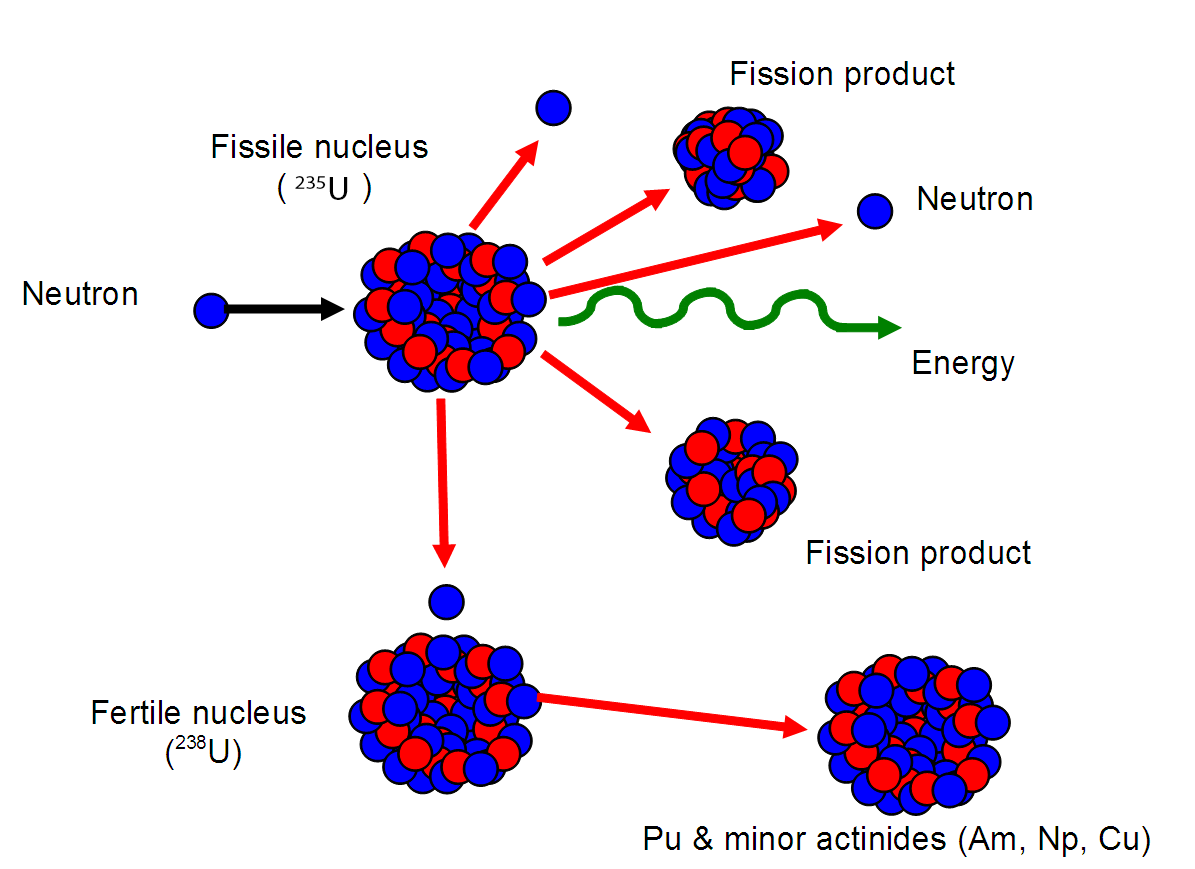
\includegraphics[width=0.8\textwidth]{pu.png}
            \caption{Schematic illustration of the two different neutron absorption processes:
            fission of uranium-235 and the radiative absorption of uranium-238. Adapted from \cite{iync_2013}}
            \label{fig:both}
        \end{figure}
    In fact, not all nuclei can undergo fission.
    Therefore, radiative capture is the only possible neutron absorption process for
    nuclei that are not fissionable.\cite{lb01}
    We will explore neutron-induced fission further in the next section. Here we give an example of radiative capture. Thorium-232, which is present in highly radioactive
    waste, has a half-life longer than the age of the universe (see Table \ref{tab:hl}). However, it can go through
    radiative capture and then subsequent beta decays to form uranium-233 (neutrinos are omitted in the equations)
    \begin{align}
        n + {}^{232}\text{Th} &\rightarrow {}^{233}\text{Th} + \gamma,\\
        {}^{233}\text{Th} &\rightarrow {}^{233}\text{Pa} + e^-,\\
        {}^{233}\text{Pa} &\rightarrow {}^{233}\text{U} + e^-.
    \end{align}
    The uranium-233 formed has a half-life of $1.4$ million years and is therefore a lot more dangerous than
    thorium-232. Another important radiative capture reaction happening inside nuclear fuel is the radiative
    capture of uranium-238 (the most abundant isotope in nuclear fuel) to form plutonium-239.
    \begin{equation}
        n + {}^{238}\text{U} \rightarrow {}^{239}\text{Pu} + \gamma
    \end{equation}
        \subsubsection{Fission and fission products}
        \label{sec:fission}
        Conjectured by Bohr and proven by Alfred O. Nier in 1939,
        the fission of uranium-235 induced by a thermal neutron
        is the best-known example of induced fission. 
        The neutron capture produces a compound nucleus ${}^{236}U$ that is in an excited state.
        Sometimes the nucleus can decay by $\gamma$ emission in capture reaction.
        But most of the time, the excitation energy deforms the nucleus into two positively charged
        parts (see Fig.~\ref{fig:fission}).
        The nucleus starts to vibrate with increasing amplitude as the kinetic energy of the
        neutron transfers to the vibrational energy of the nucleus.
        When the
        amplitude reaches a critical point, the Coulomb force overcomes the short-ranged nuclear
        force (predominantly strong force). As a result, the nucleus disintegrates into two large fragments and several neutrons.
        A typical reaction is described by
        \begin{equation}
        {}^{235}_{92}\text{U} + n \rightarrow {}^{92}_{36}\text{Kr} + {}^{142}_{56}\text{Ba} + 2 n.
        \label{eq:u235}
        \end{equation}
        Very often, photons, electrons, and neutrinos are also emitted through beta and gamma decay.
        The reaction described by Eq.~\ref{eq:u235} is not unique because different fission products can result
        from a fission.
        On average, inside a nuclear reactor, $2.5$ neutrons are produced per fission. These neutrons
        continue to induce fission of other uranium-235 nuclei, causing a ``chain reaction'' of subsequent
        fission that generate a huge amount of energy.\cite[chapt. 10]{l01}
        \begin{figure}[h]
            \centering
            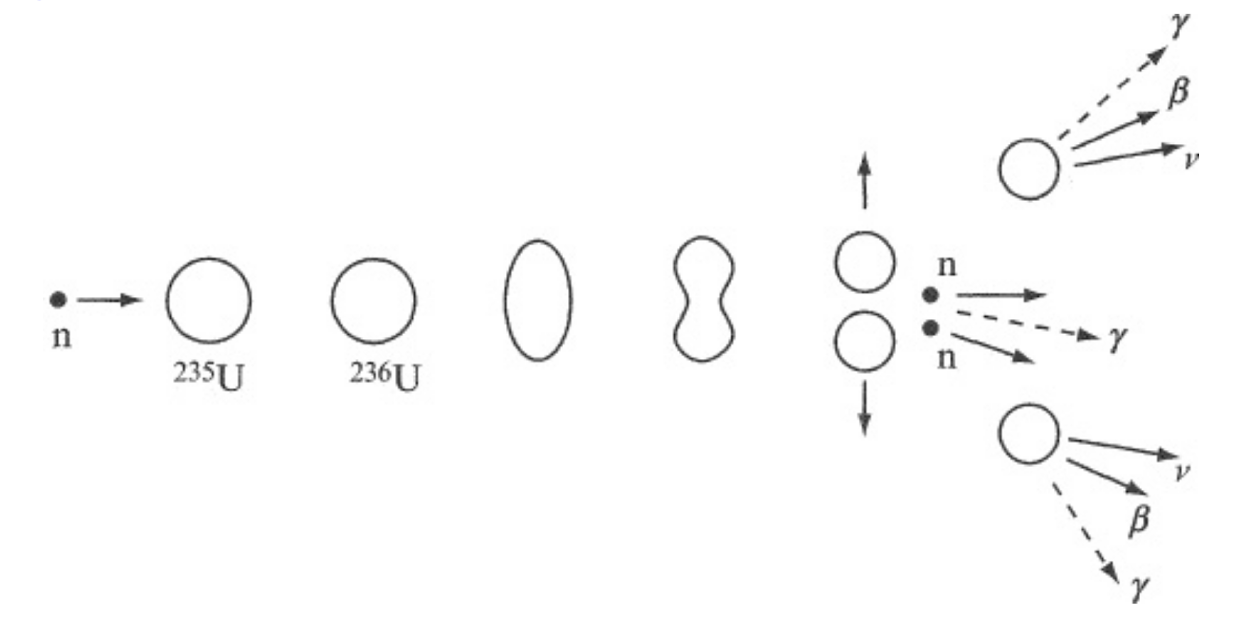
\includegraphics[width=0.8\textwidth]{fission.png}
            \caption{Illustration of the thermal neutron induced fission process of uranium-235.\cite{l01}}
            \label{fig:fission}
        \end{figure}
        \subsubsection{Fission energy}
        We can estimate the amount of energy released in fission by considering the binding energy difference
        between the parent nuclei and the fission products. As a consequence of the mass-energy equivalence in the theory
        of special relativity, we can calculate the energy released $E$ from the atomic mass differences between the parent $m_{parent}$
        and the fission products $m_{products}$.
        \begin{equation}
            E = (m_{parent}-m_{product})c^2,
        \end{equation}
        where $c$ is the speed of light.
        Essentially, any energy carried by particles that can be slowed down 
        in the reactor can be harvested as heat to generate power.

        The binding energy per nucleon is about $7.6$ MeV u${}^{-1}$ for uranium and about $8.5$ MeV u${}^{-1}$
        for a nucleus with atomic number around $117$. Hence, the change of binding energy per nucleon is
        $0.9$ MeV u${}^{-1}$, which amount to $212$ MeV for a uranium-235 atom.
        Apart from $6.5\%$ of the energy carried by the neutrinos which does not interact with the surrounding,
        the rest of the energy can be utilized by virtue of outgoing particles depositing energy in the medium
        surrounding the fuel inside the reactor.

        In reality, thermal induced fission of uranium-235 creates a variety of products and hence the energy released
        in a single reaction vary by tens of MeV. On average, about $220$ MeV per fission is recoverable for energy conversion.
        The energy generated by the fission of uranium-235 is 
        about 2.5 million times the energy produced by burning coal of the same mass.\cite{e17}

        \subsubsection{Composition and properties of spent fuel}
        Fission and radiative capture are respectively responsible for the creation of two very
        different classes of radionuclides in spent fuel
        (see Fig.~\ref{fig:spentfuel} for an illustration of the composition of spent fuel).
        \begin{figure}[h]
            \centering
            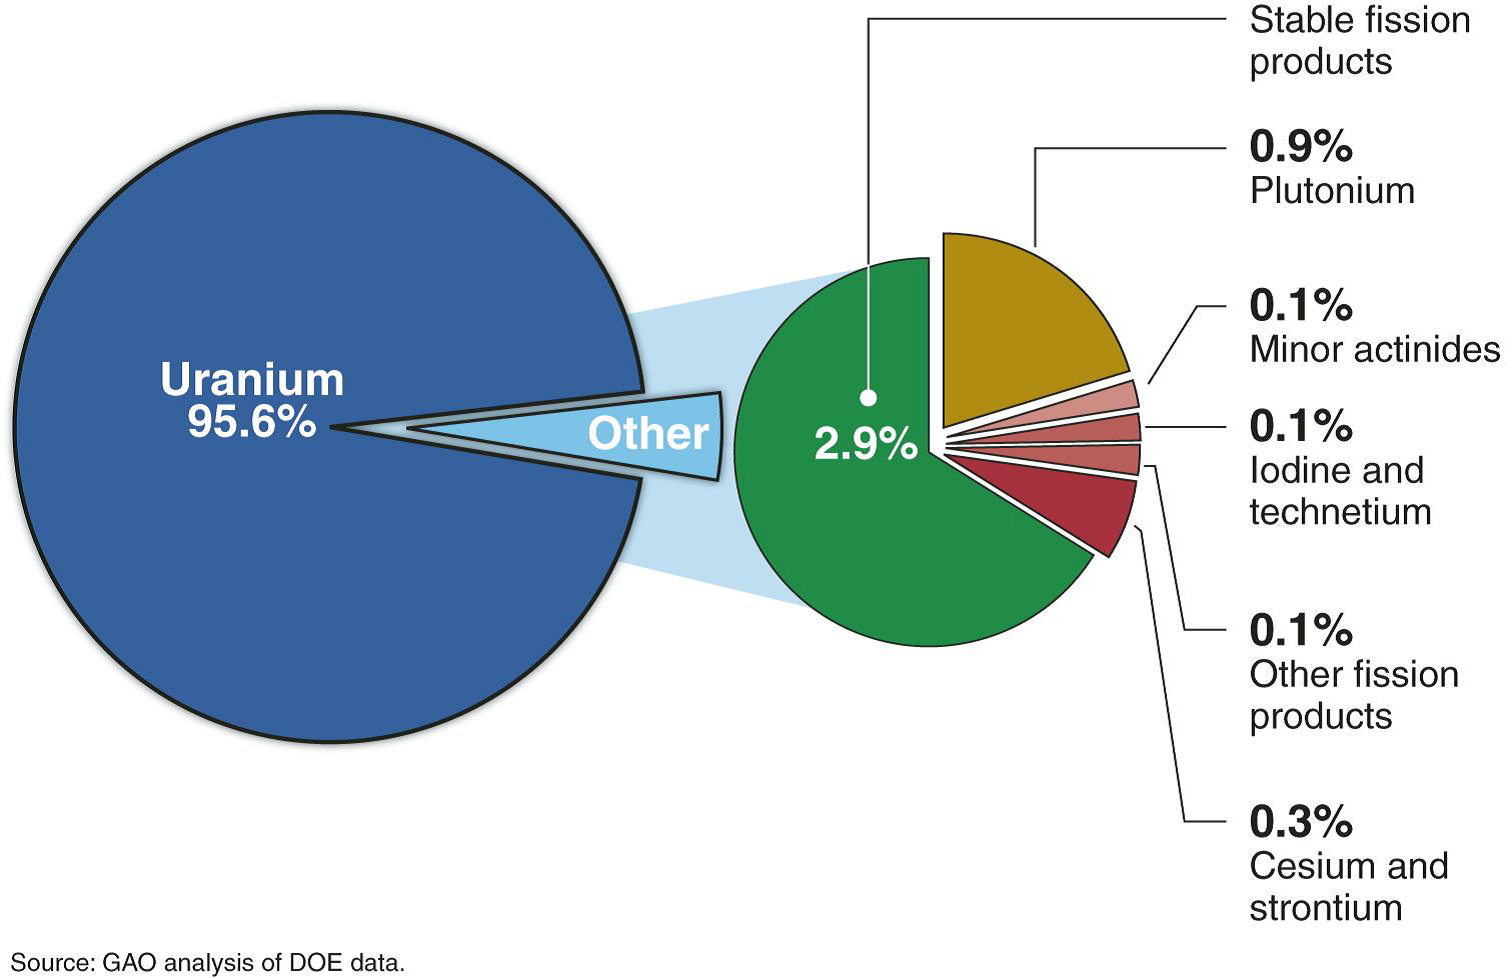
\includegraphics[width=0.6\textwidth]{spent-fuel.png}
            \caption{Composition of spent nuclear fuel for a light water reactor. The exact composition varies
            by different kinds of nuclear reactors. ``Minor actinides'' refer to transuranic elements other than plutonium.\cite{gao}}
            \label{fig:spentfuel}
        \end{figure}

        On the one hand, fission of uranium-235 produces lighter radionuclides like cesium-137 and strontium-90, which
        account for most of the short-term high activity and penetrating radiation (gamma radiation).
        In addition, for spent fuel freshly removed from the reactor, there is still a small amount ($\sim 1\%$)
        of uranium-235 left along with a lot of free neutrons released from previous fissions. Thus, a large amount
        of energy is generated via fission of the leftover uranium-235, heating up the spent fuel rods.

        On the other hand, some uranium-238 nuclei go through radiative capture
        and produce radionuclides that are
        heavier than uranium (``transuranic'') such as plutonium, neptunium, and americium.
        These transuranic nuclei have relatively low activity but their half-lives range from a few thousand years
        to a million years (see Table~\ref{tab:hl}).
        Even after a long time, their activity level remains dangerous (see Fig.~\ref{fig:csru} for
        an illustration of why this is the case).
        Moreover, these transuranic nuclei can be readily turned into plutonium-239 and proliferation is also
        an issue when one deals with these elements.
        \begin{figure}[h]
            \centering
            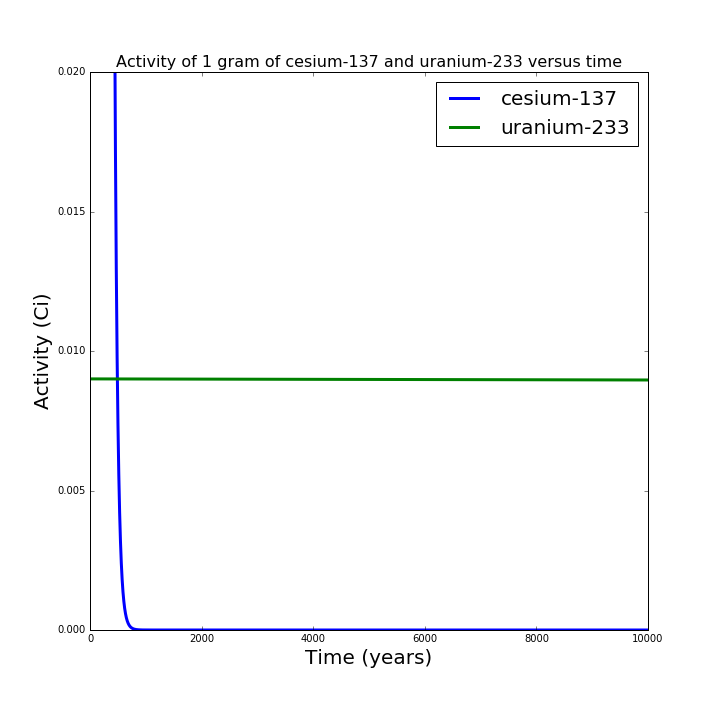
\includegraphics[width=0.6\textwidth]{csur.png}
            \caption{Activity of $1$ gram of cesium-137 (half-life $30$ years) and uranium-233 (half-life $1.3$ million
            years) as a function of time in years. The activity of cesium-137 falls off to virtually zero after a few
        hundred years; whereas the activity of uranium-233 remains about $0.01$ Ci for thousands of years. The activity
    level of $0.01$ Ci is comparable to that of the radiation source used for Computer Tomography (CT) scans.
Data from Table~\ref{tab:hl}}
            \label{fig:csru}
        \end{figure}
        Therefore, in the short term, spent fuel emits intense radiation and generates a large amount of heat.
        Moreover, in the very long term (up to millions of years), its activity still remains well above the safe level.
        The combination of these properties makes the management and disposal of spent fuel and high-level waste
        in general very difficult.

    \section{Spent fuel management}
    \label{sec:temp}
    Spent fuel from nuclear reactors is the major source of HLW.
    The concept of shielding is crucial in the short-term management of spent fuel due to the high activity
    it contains. Freshly removed spent fuel rods are stored in spent fuel pools for at least $3$ years before
    the next step. After that, reprocessing can extract the long-lived plutonium and uranium isotopes and
    convert the waste into more manageable form. However, reprocessing of commercial
    nuclear spent fuel was halted in the U.S. for cost and proliferation concerns. Instead, dry-cask
    storage, in addition to spent fuel pools, is used as an interim storage method.
    \subsection{Radiation shielding}
    Since spent fuel contains high activity, shielding of radiation is crucial. Shielding works by
    forcing the radiation to interact with the shielding medium and hence reducing the amount of energy
    the radiation carries. In the context of nuclear waste management, the most common shielding medium
    are water and concrete; and the mode of interactions of radiation with those mediums are similar to
    the physical interactions between radiation and biological molecules (the most abundant of which is
    water) described in Sec.~\ref{sec:interactions}.

    To quantify the shielding capability of a given material, we introduce cross section $\sigma$. Consider
    a beam of particles with intensity $I_i$ (with unit (area$\cdot$time)${}^{-1}$) passing through a medium
    with number density of molecules $N_s$. Suppose on average $R_i$ interactions occur per time unit.
    The cross section of the interaction between the shielding medium defined as
    \begin{equation}
        \sigma = \frac{R_i}{I_i N_s}.
    \end{equation}
    Effectively, $\sigma$ has unit of area and
    is proportional to the interaction probability of the incident radiation with a given nucleus.\cite{k88}
    Notice that the interaction probability is independent of the distance traveled by the beam in
    the medium. Written in terms of the beam intensity as a function of distance traveled $z$,
    the relationship can be expressed as
    \begin{equation}
        -\mu = \frac{d I/dz}{I},
    \end{equation}
    with the attenuation coefficient $\mu$ defined by
    \begin{equation}
        \mu = \sigma N_s,
    \end{equation}
    where $N_s$ is the number density of molecules in the medium.
    Solving the differential
    equation yields another exponential attenuation law
    \begin{equation}
        \label{eq:atten}
        I(z) = I_0 e^{-\mu z},
    \end{equation}
    where $I_0$ is the incident beam intensity. Therefore, the beam intensity decays exponentially
    with the distance traveled. Notice that $\mu$ and $z$ play symmetrical roles in the exponent. Hence
    in practice, we can trade quantity of shielding medium for the shielding capability of the type of
    molecule.

    \subsection{Spent fuel pools}
    Short-term cooling of spent fuel is necessary before further disposal or reprocessing can be done.
    Radiation shielding and cooling are the two important aspects of spent fuel pools.

    Spent fuel pools  are usually about 15-meter deep water pools,
    with storage rack at the bottom to hold the fuel assemblies. The depth ensures that the radiation
    is well attenuated by the time they reach the surface (see Eq.\ref{eq:atten}).

    The water is enriched with boron atoms that have neutron capture cross section of about $1000$ times
    the cross section of water molecule. Hence the boron atoms captures the neutrons in the spent fuel
    and prevent them from causing further fission and formation of transuranic elements.

    Additionally, the water in spent fuel pool is circulated such that heat dissipates from the spent
    fuel rods to the water via convective heat transfer. The onvective heat transfer rate in this case is
    extremely complicated and we should not try to derive it here. However, we can still gain useful insights
    from a crude approximation with the Newton's cooling law via convective transfer
    \begin{equation}
        \label{eq:cooling}
        \frac{dQ}{dt} \propto h\cdot (T_{sf} - T_{water}),
    \end{equation}
    where $Q$ denotes the heat transferred from the spent fuel to the water,
    $h$ the heat transfer coefficient (which is positive and assumed to be independent
    of the temperature), $T_{sf}$ the spent fuel temperature, and $T_{water}$ the temperature
    of the water.
    The heat transfer coefficient $h$ depends of the fluid dynamics properties of the water and can
    be measured experimentally. The goal of
    cooling is to prevent heat from accumulating in the spent fuel and thus $dQ/dt \geq 0$ at all time.
    Apply the first and third laws of thermodynamics to the spent fuel rod,
    \begin{equation}
        \label{eq:first}
        \frac{-\Delta Q}{\Delta T_{sf}} = dS > 0,
    \end{equation}
    where $Q\geq 0$ is consistent with the definition above and $S$ denotes entropy, we conclude that $Q$ and $T_{sf}$ always vary in the opposite direction. Rearrange Eq.~\ref{eq:cooling} to get
    \begin{equation}
        T_{water} \propto h\cdot T_{sf} - \frac{dQ}{dt}.
    \end{equation}
    Hence if we let $dQ/dt=0$ (its min) and $T_{sf}$ be the temperature of the spent
    fuel rods when it enters the pool (its max), we
    can obtain an upper bound on $T_{water}$, the temperature of the water. This temperature turns out to
    be about $50^{\circ}$C to transfer the heat generated by leftover fission in fresh spent fuel. After a
    certain amount of time, as the fission slows down, $dQ/dt$ decreases and hence $T_{sf}$ decreases: the spent
    fuel is cooled.

    \subsection{Reprocessing: an option}
    \label{sec:reproc}
    After spending some time in the nuclear fuel pools and cooling down, the spent fuel may be ready
    for reprocessing.
    Spent nuclear fuel contains a large amount of plutonium and uranium that are suitable as nuclear fuel
    or fissile weapon material (plutonium-239). Therefore, reprocessing the spent fuel generates plutonium and
    uranium that may be recycled. The U.S. currently does not have any commercial nuclear fuel
    reprocessing facility due to the demonstrated high cost of reprocessing
    during the West Valley Demonstration Project and water contamination issues at the Hanford Site.
    Concerns about proliferation issues also arise, as the 
    reprocessed plutonium-239 is the primary fissile element in the production of nuclear weapons.\cite{aa12}
    On the other hand, France (the world leader in reprocessing technology), India, Russia, the UK
    and China (since 2010) continues to reprocess spent fuel. To understand the details of reprocessing
    requires advanced chemistry and is beyond the scope of this work. However, the issue remains interesting
    and hence we provide an overview of the process as well as some of the related concerns.

    Almost all of the reprocessing plants use the PUREX (Plutonium Uranium Redox EXtraction) process
    to reprocess spent fuel. This process utilizes the differences in oxidation potential 
    between the heavy elements (uranium and plutonium) from the other lighter fission products.
    In this way,
    the oxidized plutonium and uranium are separated and can be reduced back to reusable radionuclides.\cite{lb01} 
    The extracted plutonium then returns to the reactor and transforms into short-lived fission products
    by fission. Un-reprocessed fuel usually takes 10 times as much time to reach the safe
    activity level ($\sim 10^5$ years) as reprocessed fuel ($\sim 10^4$ years). Moreover, since fission products
    make up a small portion of the spent fuel, reprocessing greatly reduces the mass of the waste. The reprocessed
    waste can be turned into liquid form, mixed with frit (the substance from which glass is made) and then
    vitrified (made into glass). The vitrification process immobilizes the radioactive particles and makes
    the waste much more safe and manageable, but vitrification can only be applied to reprocessed spent fuel.

    It is worthwhile to note that the PUREX processed was designed specifically to separate plutonium for
    bombs. Therefore, literally any other reprocessing approach would be less prone to proliferation.
    Researchers are actively investigating alternatives to the PUREX technology. For example, the UREX+ (for
    uranium extraction) technique extracts the uranium but leaves the plutonium mixed with other
    radioactive materials.\cite{aa12}

    \subsection{Dry cask storage}
    Spent fuel pools have very limited capacities. 
    In the case where the spent fuel is not reprocessed, overground dry cask storage provides a low-cost temporary storage before the spent fuel is disposed of.
    After cooling in the spent fuel pools for at least a year, the spent fuel can be stored in dry casks filled with inert gas. 
The dry casks are often metal cylinders welded to prevent leakage. Each cask is surrounded by
    additional steel and concrete to provide shielding.
    The heat from the cask is removed by passive
    cooling (air circulation). The NRC is hoping that the casks will
    last safely for as long as 100 years, yet it has been observed that corrosion and cracking can occur in 30 years
    or less.\cite{aa12} As such, without the prospect of a permanent geological repository,
    overground dry cask storage does not seem to be a long-term solution.
    Even more striking is the fact that more than $75\%$ of the spent fuel is still stored in densely
    packed pools
    that are close to or over their limiting capacity.\cite{a11,aa12}
    Therefore, there is clearly a need for a long-term disposal plan.

\section{Disposal of HLW}
\label{sec:disposal}
    The time frame of nuclear waste disposal is about $10^4-10^6$ years, after which the radioactivity
    of the waste is predicted to decline to a safe level (see Sec.\ref{sec:waste:spentfuel}).
    Deep geological repositories that are stable over geological timescales naturally offer a good option for disposal.
    In fact, it is accepted by the international science community that geological repositories in a stable environment over 300 meters underground 
    is safer than indefinite overground storage of HLW, reprocessed or not, as above-ground storage
    is susceptible to catastrophic events like earthquakes and human-caused
    threats like terrorist attacks.\cite{fmr11}
    In this section, we first use Yucca Mountain Nuclear Waste
    Repository     as a case study to understand the requirements for a permanent HLW disposal site.
    Then we look at an alternative to a permanent deep geological solution:
    deep boreholes storage.
        \begin{figure}[h]
            \centering
            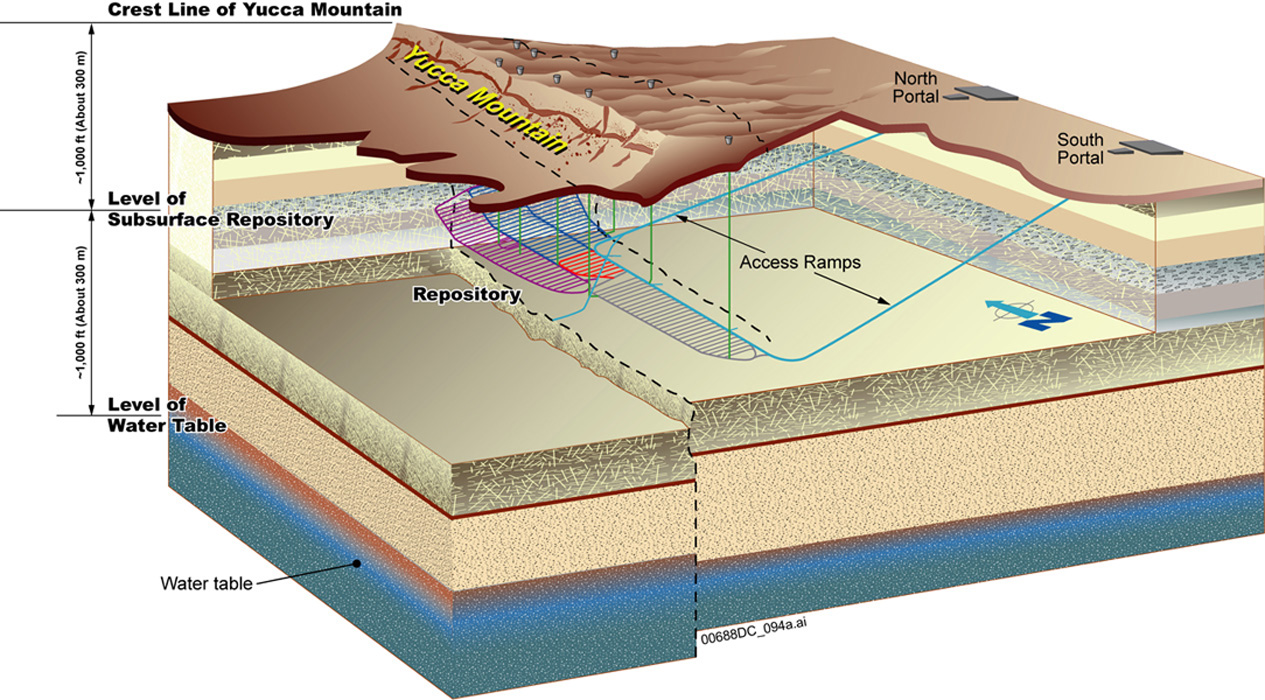
\includegraphics[width=\textwidth]{yuccaRepo.jpg}
            \caption{Design of the 300-meter deep Yucca Mountain Waste Repository.\cite{yucpic}}
            \label{fig:yucca}
        \end{figure}
    \subsection{Deep geological repository: Yucca Mountain}
        The defining characteristic for a nuclear waste disposal site is its ability to minimize human
        exposure to radiation over the next ten thousand to a million years or more.
        For a deep geological repository, this means preventing the release
        of radionuclides to the ground water or the surface.
        Due to the amount of radiation the repository would contain, it would be difficult to perform
        maintenance once the waste was deposited. Therefore, scientists and engineers are challenged
        to predict the geological environment of Yucca Mountain over the next one million years and come up
        with a design that they will have very little chance to alter once it is implemented.

        The Yucca Mountain Nuclear Waste Repository was designated by the Nuclear Waste Policy Act
        of 1987 to be the nation's permanent deep underground repository for spent nuclear fuel. It is
        located near the Nevada Nuclear Weapon Test Site.
        It is located 300-meter under the peak of Yucca mountain with impermeable layers of rocks
        separating the repository
        from both the surface and the ground water (see Fig.~\ref{fig:yucca}).

        The project has been highly contested since its
        inception and the Obama administration ended federal funding for the project in 2011, citing political,
        not safety or technical, reasons. We will take a glimpse at the suitability assessment of the site
        as a nuclear waste repository to get a sense of its technical complexity.

        \subsubsection{Geological stability of Yucca Mountain\footnote{This section is a short summary of \cite{m06}}}
        The chief concern of the suitability of Yucca Mountain was about water. If moist air comes to
        contact with the waste, the waste may get oxidized and become chemically and physically unstable, thereby
        releasing radionuclides.
        The community seemed to agree that the packaging will have to carry the primary
        responsibility of preventing the oxidation of the waste, but predicting the performance of some
        engineered product over the timescale of a million years is not something with which we have had much 
        experience. Over time, the radiation from the waste will also alter the rock (by altering its composition
        and creating fractures) and hence the water percolation rate.

        Many other factors are considered. Climate change will influence precipitation and thus the
        rate at which water percolates the rock and reaches the waste. 
        Tectonic motion may change how much the rocks are fractured and thus the percolation rate.
        Volcanic activity, meteorite strike and earthquakes may seriously undermine the integrity of the repository.
        Hot upwelling water from below the repository may corrode the packaging and release radionuclides into
        the ground water system. It is impossible to address all of these concerns in this work, but we will look
        at how the risk assessment is carried out in the case of volcanism.

        \subsubsection{Total System Performance Assessment (TSPA)}
        The Department of Energy (DOE) created Total System Performance Assessment (TSPA) as a complicated
        probabilistic
        computer model that predicts the potential annual dose to the potential receptor.
        Essentially, the TSPA takes a huge set of parameters characterizing features that DOE deems as important,
        carries out geophysical and geochemical simulations,
        and outputs the expected annual dose leaked from the repository.
        DOE expects that
        uncertainty is fully integrated into the analysis done by TSPA such that even if the model itself change
        (for example if new parameters and factors are included), the results from TSPA will not change
        significantly.\cite{cv14,ocrwm02} 

        \subsubsection{Risk and uncertainty estimation: volcanism}
        \label{sec:volcano}
        Yucca Mountain is composed of volcanic rocks created from a series of large-volume eruptions between
        fifteen million and eight million years ago. However, it is the small-volume eruptions, the last of
        which occurred about $75,000$ years ago, that would the most likely pose risk to the repository
        in its life span of a few million years.
        The central question is whether the risk of volcanic eruption is acceptable. Mathematically,
        according to the Environmental Protection Agency (EPA)'s 1993 guideline,
        if the probability of a volcanic eruption seriously damaging the repository is less than
        one in ten million per year, it is acceptable.\cite{epa93}
        Of course, one has to also consider consequences of a potential radiological releases if an eruption
        occurs. Here we focus on the estimation of occurrence probability.

        The probability that a future volcanic eruption disrupting a repository over
        the repository's lifetime is given by
        \begin{equation}
            \label{eq:prob}
            P(D) = P(E2|E1)P(E1),
        \end{equation}
        with the standard probability notation: 
        $P(A)$ means probability of event $A$ happening;
        $P(A|B)$ gives the probability of event $A$ happening given that event $B$ happened;
        $D$ denotes the disruption event,
        $E2$ the event that the eruption affects the repository, $E1$ the event that an eruption occurs.
        Essentially, we are looking at the probability of a volcano occurring and affecting the repository.

        The information necessary to estimate the probability is listed in the flowchart Fig.~\ref{fig:volcanos}.
        The boxes represent decision parameters that depends on the judgment of the decision makers and
        the scientists. For example the ``Volcanic Zone Models'' should be picked by the scientists, and
        ``Repository Area'' decided by policy makers.
        
        The ovals are probabilistic parameters in which uncertainty
        is represented as a probability distribution over a range of possible values.
        Each oval is a complex computational model.
        The large bold ovals are the $E1$ and $E2$ parameters in Eq.\ref{eq:prob}.
        The $E2$ oval makes
        use of the events simulated in $E1$ to calculate the conditional probability $P(E2|E1)$ and output
        the disruption probability $P(D)$ to TSPA, which calculates the expected leaked dose over the
        life span of the repository. Here we look in some detail at the calculation of those parameters.
        \begin{figure}[h]
            \centering
            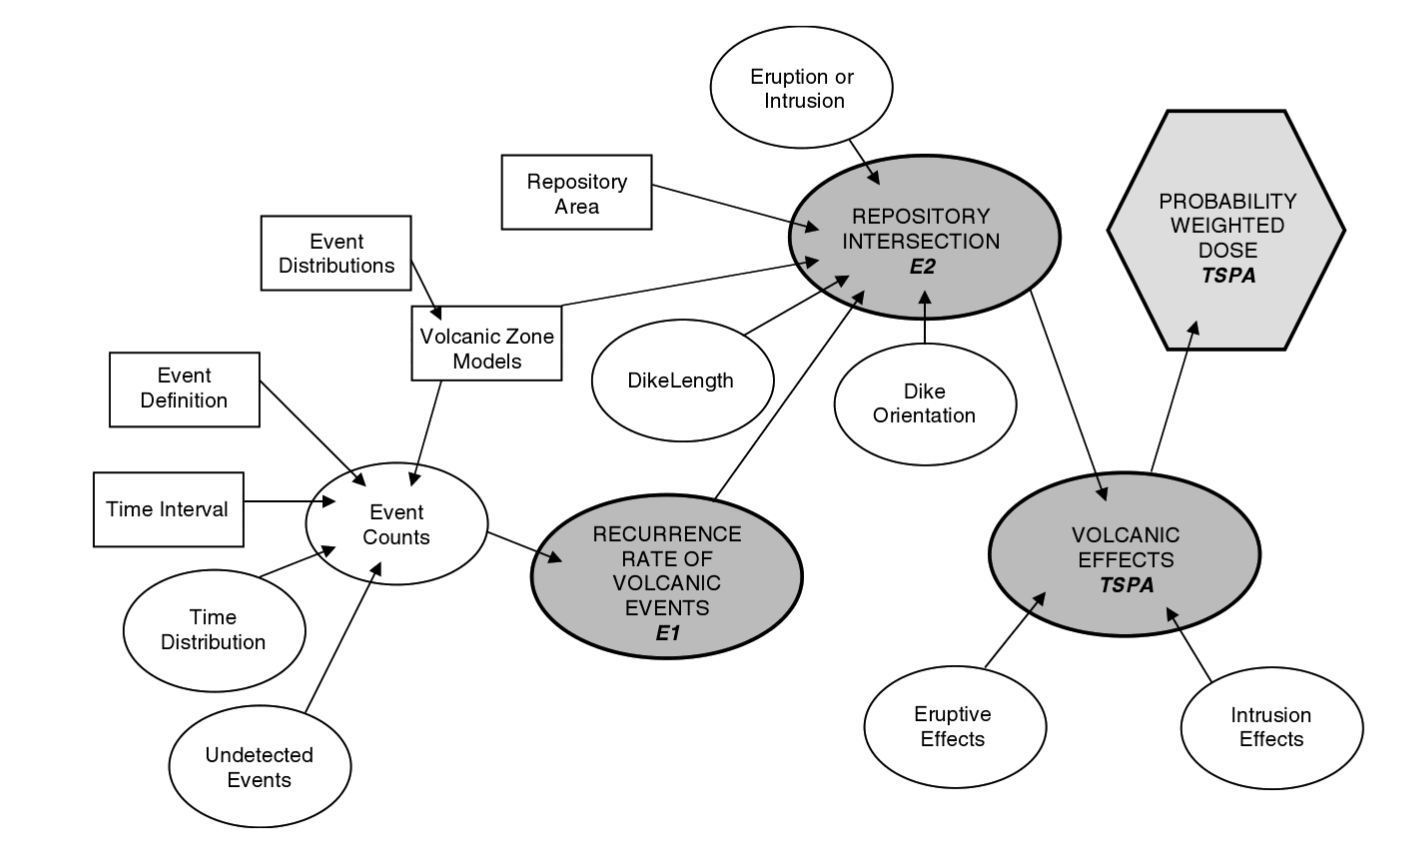
\includegraphics[width=0.9\textwidth]{volcano.png}
            \caption{A flowchart for the volcanism risk estimation problem. The oval-shaped
            boxes are probabilistic models, hexagon shaped the TSPA computational model, and
        square human decisions.\cite{cv14}}
            \label{fig:volcanos}
        \end{figure}

        \paragraph{Monte-Carlo simulation}
        Estimation of uncertainty is key in this problem, because over the timescale of a million years,
        a small uncertainty would amount to large measurable change. Recall the traditional method of
        propagation of uncertainty. Let $\delta_X$ denote the uncertainty in variable $X$. For a function
        with analytic form $y(x_1,x_2,...x_n)$, the uncertainty in $y$ is given by
        \begin{equation}
            \delta_y = \sqrt{\sum\limits_{i=1}^n \left(\left.\frac{\partial y}{\partial x_i}
            \right\rvert_{x_i} \delta_x\right)^2},
        \end{equation}
        which uses a linear approximation of $y(x_1,x_2,...,x_n)$ near the measured values of
        $(x_1,x_2,...,x_n)$.
        However, if the uncertainty of the input parameter is expressed as a distribution, or if $y$ is
        not an analytic function, then the propagation of uncertainty method fails. In our volcano disruption
        problem, $y$ can be seen as the complex computational model like TSPA. However, there is a
        straightforward algorithm called Monte-Carlo simulation that can estimate the uncertainty of $y$.
        The steps of the algorithm is as follows.
        \begin{itemize}
            \item Generate a large number of $(x_1,x_2,...x_n)$ samples according to their respective distributions.
            \item For each $(x_1,x_2,...,x_n)$ sample, calculate a $y$ value (with the computational model).
            \item Aggregate all the $y$'s generated to estimate its distribution or uncertainty.
        \end{itemize}
        This method usually converges reasonably fast -- the error goes down as $1/\sqrt{N}$ where $N$ is the number
        of samples generated. It is the algorithm of choice in Fig.~\ref{fig:volcanos} to
        propagate the uncertainty information in one oval to another.
        \paragraph{Recurrence rate} The recurrence rate $E1$ only uses information from the ``Event Count''
        oval, which estimates the true number of eruptions in the Yucca Mountain region in a given time range
        from observed data. The choice of time range is not trivial: longer time range certainly gives us
        more data and hence improved statistics, but longer time interval dated far back may fail to represent
        future event rates since the geology evolves. The best approach seems to be choosing the time interval
        based on geological cycles.

        Finally, we need the undetected volcanic intrusion rate to establish the recurrence rate. Volcanic
        intrusions are essentially underground eruptions that can go undetected. The DOE field studies conclude
        that intrusions are possible but are presumed to be associated with surface eruption in space and time. 
        By contrast, the NRC argues that intrusions need not be associated with eruption and there
        may be three to five times as many undetected intrusions as detected surface eruptions. The divergence
        of the two agencies' viewpoints partly attributes to their different estimated recurrence rate.
        From different studies adopting different input models, estimated recurrence rate ranges from
        $1.5\times 10^{-6}$ to $8\times 10^{-6}$ events per year. These estimates translate to an estimated
        time between events from 125 thousand years to 250 thousand years. We can see that the choices of
        models introduce a significant uncertainty to the estimation.\cite{cv14}

        \paragraph{The probability of repository intersection}
        Given a probability distribution for $E1$, we can estimate $P(E2|E1)$ -- the probability of
        a given event intersecting the Yucca Mountain site per year assuming that it is independent
        of time. It is simply the ratio of the area of
        the repository to the entire volcanic zone of a given event. Since the area of the repository
        has not been decided, a probability distribution over a range of areas is used.
        However, since not enough volcano events have been observed in the region, the model
        to predict the size of the volcanic zone is not well determined.
        Different models predict $P(E2|E1)$ ranging from $0.015$ to $0.0008$ per year, which again has a high
        uncertainty.

        \paragraph{The probability of a disruption} The probability distribution of $E1$ and $E2$
        are combined through a Monte-Carlo simulation to produce the disruption rate $P(D)$
        at the Yucca Mountain repository. DOE estimates a mean disruption rate of $1.5\times 10^8$ events
        per year with
        a 90 percent confidence interval of $5.4\times 10^{-9}-4.9\times 10^{-8}$ events per year. Hence the DOE's result
        states that most likely the disruption won't happen more than once every 20 million years.

        The NRC emphasizes the importance of the risk assessment nature of the problem and uses only a subset
        of the DOE model that reflect conservatism. It concludes a disruption rate of
        $10^{-7}$ to $10^{-8}$ per year. Furthermore, it argues that it should not distinguish the likelihood
        of disruption rate of different values within this range. Therefore it picks the upper bound
        of $10^{-7}$ as the estimated event rate, representing the worst case estimate.

        Both the NRC and the DOE conclude with a very low volcanic disruption rate that is below the EPA
        $10^{-7}$ events per year threshold of negligible risk.
        Nevertheless, the consequences of such a disruption event is still not well understood.
        If the leaked dose is low in such an event, then the risk is negligible. If the leaked dose is high,
        then the NRC estimate of $10^{-7}$ events per year would necessitate further investigation into such
        a scenario.\cite{cv14}
        \subsection{Deep borehole disposal}
        Deep borehole disposal utilizes deep and narrow boreholes to dispose of HLW. The boreholes
        will place the packaged waste as much as 5 kilometers under the surface of the ground and seal it
        with concrete clay.
        The engineered packaging, along with the granite rock with few cracks on which the borehole is drilled,
        provides
        good isolation for the radionuclides in the waste (See Fig.~\ref{fig:borehole}).
        \begin{figure}[h]
            \centering
            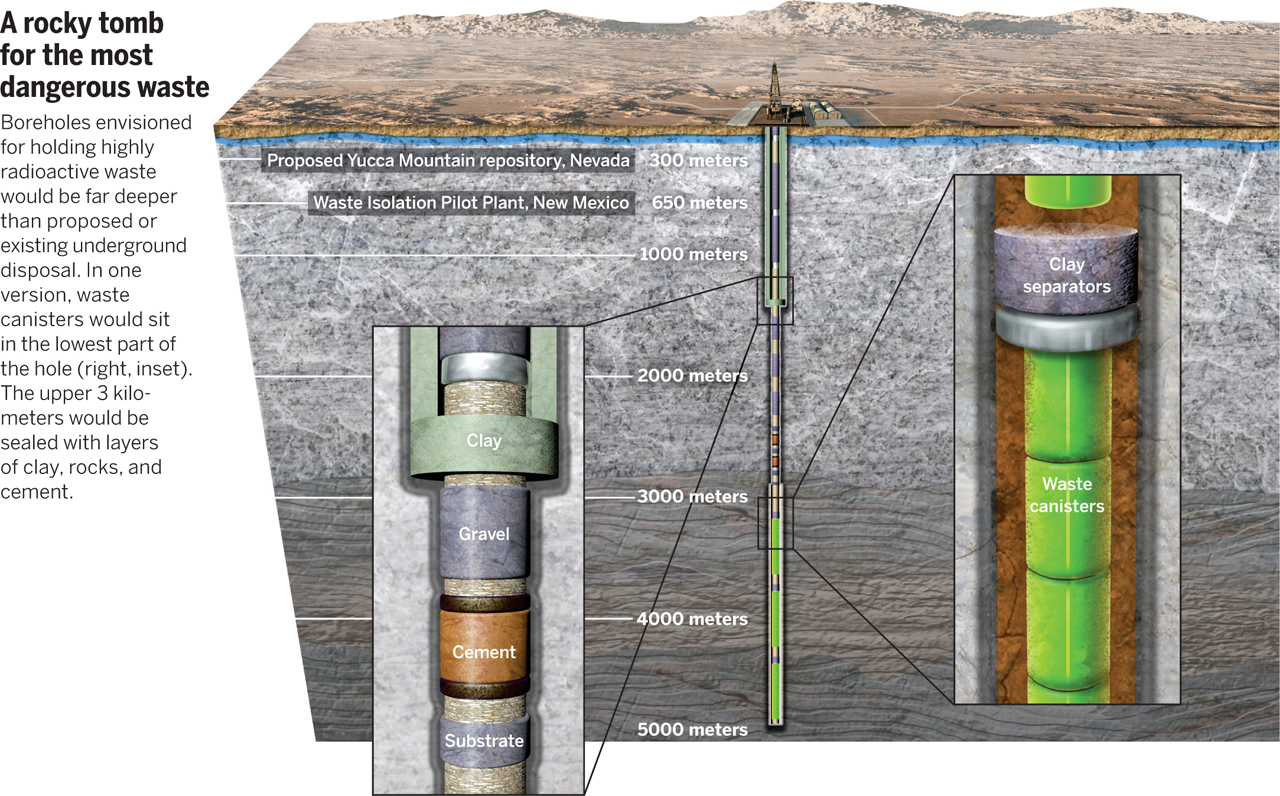
\includegraphics[width=0.8\textwidth]{borehole.jpg}
            \caption{Illustration of borehole disposal, with deep repositories' depths for comparison.\cite{c15}}
            \label{fig:borehole}
        \end{figure}

        Deep boreholes have several advantages over deep geological repository. For example, suitable
        rocks can be more readily found for boreholes (since it does not take up a lot of space and can be
        of smaller scale),
        whereas large repository sites are hard to identified. \cite{b09,c15}
        However, the borehole solution has its own limitations.
        Drilling a hole as deep as 5 kilometers poses a daunting engineering challenge.
        Moreover, reactor rods from commercial nuclear plants in the U.S. usually size up to 2 meters in diameter,
        which would be too large for the borehole and require extensive repackaging.
        Nevertheless, deep borehole disposal remains a valid option.
        Sandia lab has embarked on a five-year plan to experiment with the deep borehole design.\cite{c15}

\section{Discussions}
Nuclear waste management and disposal is certainly becoming an increasingly pressing issue.
We explore the creation, management and disposal of highly radioactive nuclear waste and the physical
principles underlying those processes. The increasingly over-packed spent fuel pools and the challenges
associated with geological repositories are the weak links in this chain.

In terms of scientific analyses for a geological repository, much has yet to be done.
On the performance analysis end, we need
to think about how to model without enough data and how to deal with orders of magnitude uncertainty.
Perhaps some other analysis methods are required. Building and comparing the performance of 
small retrievable repositories that store
nuclear waste for about 100 years may give us insights on the stability of different geological sites.

Newer reprocessing methods (as mentioned in Sec.~\ref{sec:reproc}) are being proposed
as  solutions to the proliferation issue from the current reprocessing method.
 Reprocessing techniques can significantly reduce the volume of the waste and make it more
manageable. With reprocessing, deep boreholes storage may become a more feasible disposal solution 
for commercial reactor waste. 

%\begin{acknowledgments}
%Thanks Joel and peeps. Arjendu and M. V. Ramana.
%\end{acknowledgments}
\newpage
\bibliographystyle{aip}
\bibliography{refs}
%\newpage
%\appendix
%\section{Derivation of Fermi's Golden Rule \#2}
%\label{a:fermi}
\end{document}
